\documentclass{article}
\usepackage{longtable}
\usepackage{geometry}
\usepackage{hyperref}
\usepackage{graphicx}
\usepackage{float}
\usepackage{cite}
\linespread{1.2}

\begin{document}
\begin{titlepage}
    \centering
    % Add your title, author, date, and other information here
    
\includegraphics[scale = 0.6]{logo.jpg}
    \\---------------------------------------------------------------------------------------------------------------------------------
    \vspace{0.5cm}
    \\\huge\textbf{Waste Classification through Image Processing}\par
    \vspace{0.5cm}
    \Large{CS 446: App. Digital Image Processing}\par
    \vspace{1.5cm}
    \large\textbf{Members:}
    \\ \large{Zainab Haider - 07104}
    \\ \large{Bushraa Yousuf - 07609}
    \vspace{0.5cm}
    \\\large\textbf{Instructor:}
    \\\large{Dr. M. Mobeen Movania}
    \vspace{0.5cm}
    \\\large\textbf{Section:}
    \\\large{L1}
    \vspace{1.7cm}
    \\\large{From the department of Computer Science}
    \\\large{Dhanani School of Science and Engineering}
    \\\large{Habib University}
    \\\large{\today}
\end{titlepage}

\tableofcontents
\vspace{7.3cm}
\section{Introduction}
    In our urbanized world that is changing rapidly, environmental concerns are emerging at a fast pace. Efficient waste management system are in now needed more than ever. In our project, "Waste classification through Image Processing," we aim to address this pressing issue by harnessing the power of applied image processing. We will be using MATLAB and CNN for this project.
    \\
    MATLAB, a powerful and versatile software, can help us significantly to classify different materials and in waste through image processing. It can optimize the images of garbage, like adjusting lighting conditions, standardizing image sizes. This preprocessing of images can help us in the next step, which is to extract relevant features from sample images. This include color information, texture patterns, and shape characteristics of the waste materials. MATLAB's extensive toolbox provides a wide array of image processing functions, filters, and algorithms, making it possible to capture the unique visual attributes of different waste types.
    \\
    MATLAB serves as a versatile platform for training machine learning models, particularly Convolutional Neural Networks (CNNs), by utilizing the valuable image features extracted from waste material images. CNNs are specialized deep learning models designed to excel in image analysis tasks. They function like sophisticated detectives, scrutinizing the visual nuances of waste materials. With the extracted image features as clues, CNNs can discern subtle differences between various waste types based on their unique visual signatures. MATLAB organizes an iterative training process for these CNNs, refining the classification model through multiple rounds of learning and evaluation. This iterative approach allows the CNN model to continuously improve its ability to accurately identify and differentiate waste materials. 
\section{Motivation}
    In a world confronted by flourishing urbanization and escalating environmental concerns, the significance of waste management cannot be overstated. It is an issue that affects us all, with far-reaching implications for our environment, public health, and resource conservation. However, traditional waste management systems often struggle to keep pace with the increasing volume and complexity of waste generated daily. This is where our project, "Waste Classification through Image Processing," fueled by machine learning models and image processing, steps in to make a profound impact.

Efficiency and Automation:
One of the primary motivations behind our project lies in the quest for efficiency and automation in waste management. Conventional waste sorting methods are labor-intensive, prone to errors, and often inefficient. By harnessing power of neural networks, we aim to automate the process, significantly reducing the reliance on manual labor and the associated costs. Through image processing techniques, our system can rapidly and accurately classify waste materials, making waste sorting a streamlined and efficient operation. This, in turn, enables waste management facilities to allocate their resources more effectively and achieve substantial cost savings.

Environmental Impact:
The environmental imperative is another compelling reason driving our project. Inefficient waste management contributes to environmental degradation through increased landfill usage and contamination of natural ecosystems. This Software-based waste classification can improve recycling rates and ensure that materials are disposed of properly, thus reducing the strain on landfills and mitigating the harmful effects of waste on the environment. By addressing these issues, our project strives to foster a more sustainable approach to waste management, safeguarding the delicate balance of our ecosystems and enhancing the quality of life for all.

Data-Driven Decision-Making:
Crucially, our project is motivated by the potential of data-driven decision-making. We can use AI based data analysis systems excel in analyzing vast amounts of data, and waste management is no exception. By collecting and processing data related to waste generation and management trends, our project empowers authorities and organizations with the insights needed to make informed decisions. This includes optimizing waste collection routes, tailoring recycling programs to specific needs, and efficiently allocating resources where they are needed most. Through data-driven strategies, we aim to transform waste management from a reactive process into a proactive, sustainable, and cost-effective endeavor.

In conclusion, "Waste Classification through Image Processing" is not just a project; it's a commitment to a cleaner, more sustainable future. By prioritizing efficiency, reducing our environmental footprint, and leveraging data-driven insights, our project is poised to revolutionize waste management practices. It is a testament to our dedication to addressing one of the most pressing challenges of our time and contributing to a healthier, more sustainable planet for generations to come.
\section{Novel Idea}
Our project, "Waste Classification through Image Processing," is novel due to its utilization of machine learning models and image processing to transform waste management. In contrast to conventional manual sorting techniques, our automated system employs sophisticated algorithms to precisely categorize waste materials in real-time, resulting in increased efficiency and decreased errors. This innovative method holds the promise of substantially elevating recycling rates, minimizing environmental harm, and optimizing resource allocation, establishing it as a pioneering solution within the waste management domain.

\section{Mathematical Model}
For image classification, we will be using CNN(Convolutional Neural Network). CNN is made up of different layers. Below is the standard mathematical model for the different layers of CNN:
\begin{enumerate}
    \item \textbf{Convolutional layer}
    \\ 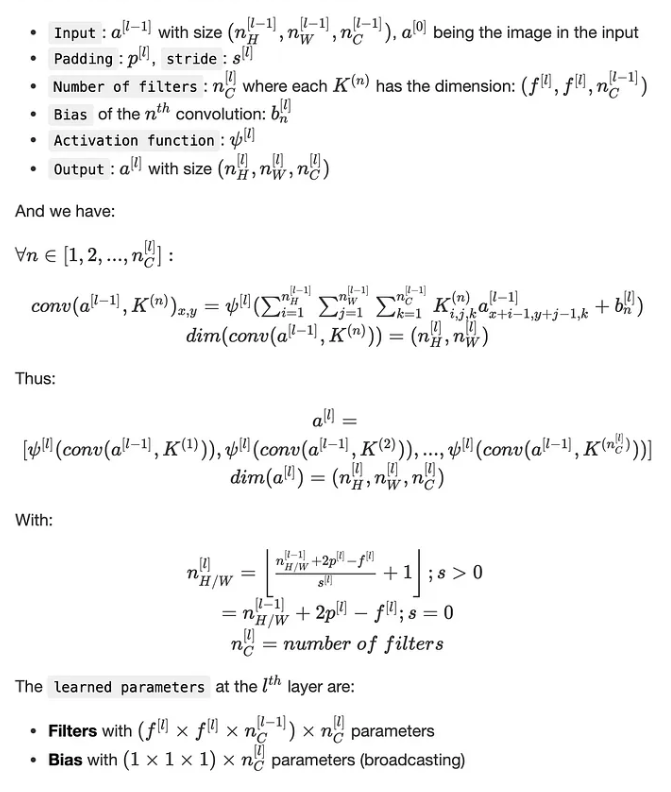
\includegraphics[scale = 0.6]{1st.png}
    \item \textbf{Pooling layer}
    \\ 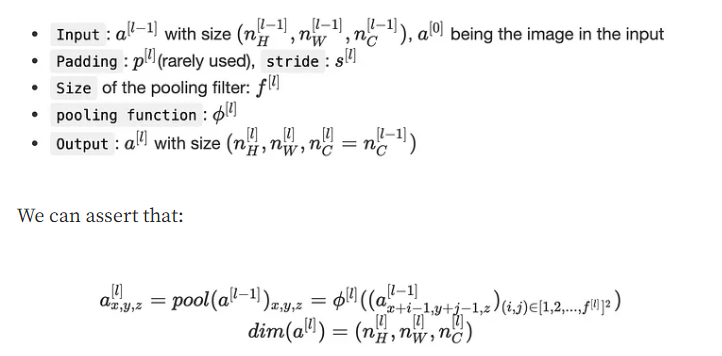
\includegraphics[scale = 0.69]{2nd.png}
    \item \textbf{Fully connected layer}
    \\ 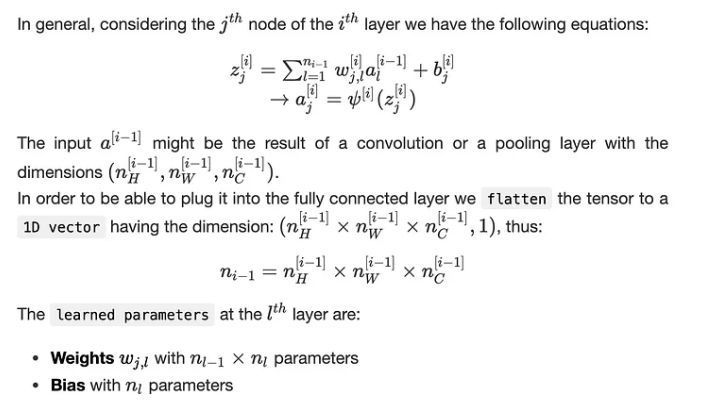
\includegraphics[scale = 0.69]{3rd.png}
\end{enumerate}
The following illustruation can sum up the the working of these layers:
\\ 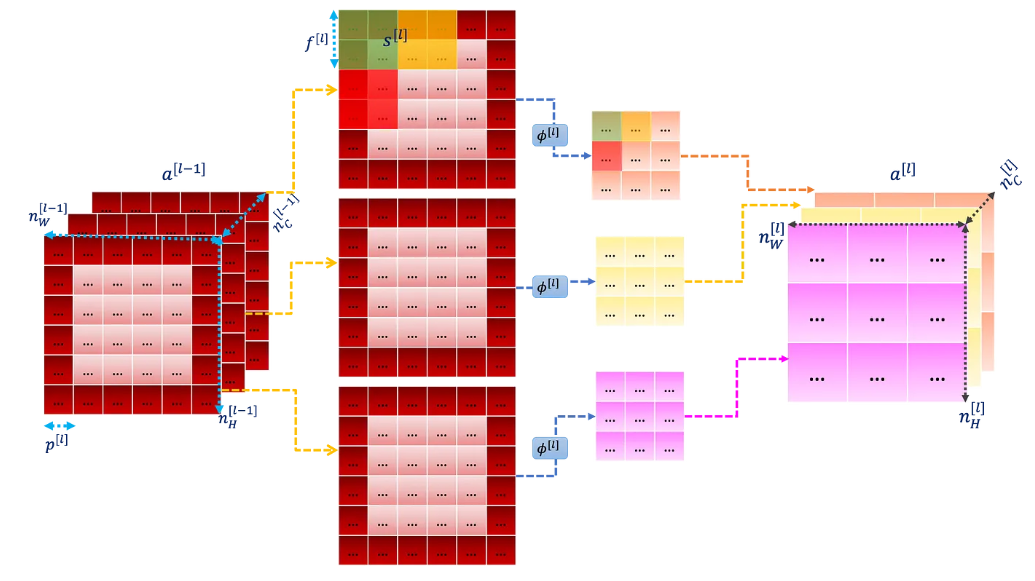
\includegraphics[scale = 0.55]{4th.png}    
\section{Relevance in Local Context}

Pakistan grapples with a significant solid waste management challenge, producing a staggering 49.6 million tons of waste annually, a number increasing at a rate of over 2.4 percent each year. Unfortunately, only a meager 13 to 23 percent of this waste is recycled due to the absence of a well-established recycling industry and the predominant reliance on manual sorting methods.

In this landscape, the development of a project like ours, focusing on efficient garbage classification, stands as a pivotal step towards addressing these issues. Introducing advanced waste sorting technologies and processes serves as a stepping stone in the foundation for a much-needed recycling industry in Pakistan. Such an industry holds multifaceted benefits for the nation.

Furthermore, a thriving recycling industry can play a pivotal role in reducing environmental pollution. By diverting a significant portion of waste from landfills and incineration, it minimizes harmful emissions and prevents soil and water contamination. This translates into cleaner air, water, and land for urban and rural areas. Additionally, recycling conserves valuable natural resources, reducing the need for the extraction and processing of new raw materials. This not only eases the strain on ecosystems but also lowers energy consumption, contributing to a more sustainable and eco-friendly future for Pakistan.
\section{Project Plan}
The table below gives the tentative project plan we will be following:
\begin{center}
\begin{table}[H]
\centering
\begin{longtable}{|c|p{0.6\textwidth}|c|}
\hline
Phase & Description & Duration \\
\hline
Literature Review & Our research initiative involves a comprehensive review of existing work on our chosen topic, comparing various approaches. A key focus is studying Convolutional Neural Networks (CNNs) for image classification, dissecting their architectures and performance metrics. Through this analysis, we aim to find new ways to contribute to this field, ultimately finalizing our project plan. & 2 weeks \\
\endfirsthead
\hline
Image Processing and implementation & Our next phase of the project involves delving into the image processing component. We will begin by gathering the necessary data for our research, followed by the implementation and training of our Convolutional Neural Network (CNN) model. Rigorous testing will ensue to evaluate its performance. Concurrently, we'll actively seek opportunities to refine and enhance the model's functionality, ensuring it aligns seamlessly with our project goals. & 6-8 weeks \\
\hline
GUI interface implementation & In the project's final stage, we'll develop a user-friendly GUI, emphasizing a sleek appearance and ease of use. This essential step will ensure a polished and inviting interface, aligning our project with user expectations and marking its completion. & 2 weeks \\\hline
\end{longtable}
\end{table}
\end{center}

\section{Team Distribution}
As there are only two individuals in our group, we will collaborate closely on most tasks, and the workload will be shared evenly between us. The table below gives deatils on the work distribution:\\ \\ 
    \centering
    \begin{tabular}{|c|c|}
        \hline
        Member & Distribution         \\ \hline
        Zainab Haider    & 50\%   \\ \hline
        Bushraa Yousuf    & 50\%  \\ \hline
    \end{tabular}
\begin{thebibliography}{9}
  \bibitem{GeeksForGeeks}
  International Trade Administration. \textit{} [Online]. Available: https://www.trade.gov/country-commercial-guides/pakistan-waste-management
  
  \bibitem{Brilliant}
  Dawn News. \textit{} [Online]. Available: https://www.dawn.com/news/1505436.
  \bibitem{Brilliant}
  Arab News. \textit{} [Online]. Available: https://www.arabnews.pk/node/1894661.
  \bibitem{Brilliant}
  Medium. \textit{} [Online]. Available: https://towardsdatascience.com/convolutional-neural-networks-mathematics-1beb3e6447c0.
 
    \end{thebibliography}
\end{document}
